% * ─── CHAPTER 4 ────────────────────────────────────────────────────────────────
\chapter{Evaluation}\label{EVAL}

This chapter presents the evaluation of Climatica.
Section~\ref{EVAL_DEMO} demonstrates the application through two representative
usage scenarios drawn from forest management practice.
Section~\ref{EVAL_METHOD} describes the evaluation methodology and study design.
Section~\ref{EVAL_PARTICIPANTS} profiles the participants.
Section~\ref{EVAL_SUS} reports the usability results derived from the System
Usability Scale.
Section~\ref{EVAL_QUAL} analyses the open-ended feedback.
Section~\ref{EVAL_DISCUSS} discusses the results, acknowledges limitations,
and identifies directions for future work.

% * ─── 4.1 Demo Scenario ───────────────────────────────────────────────────────
\section{Demo Scenario}\label{EVAL_DEMO}

This section demonstrates Climatica through two representative usage scenarios
drawn from forest management practice, suggested by Prof.\ Dr.\ Felipe Bravo,
Catedrático de Planificación Forestal at the Universidad de Valladolid and
Director of the Sustainable Forest Management Research Institute (iuFOR).

Both scenarios involve domain specialists --- forest managers and ecologists
--- who need to interpret historical climate data to support practical
decisions. While these users possess deep knowledge of forest ecosystems and
climate science, they typically lack the GIS or programming background
required to query WorldClim raster files directly, making an application like
Climatica particularly valuable for their workflows.

\subsection{Scenario 1: Updating a Forest Management Plan}\label{EVAL_DEMO_FMP}

\subsubsection{Context}

Forest management plans (FMPs) traditionally incorporate an assessment of the
local climate over the preceding 30-year period. This baseline informs
decisions about species selection: which tree species are appropriate for a
given site is determined in part by the temperature range, precipitation
regime, and aridity of that location. Under a stable climate, a plan valid
today would remain valid for the life of the forest stand.

Climate change has disrupted this assumption. Mean temperatures across the
Iberian Peninsula have risen by approximately 1.5\,$^\circ$C over the past
50 years~\cite{ipcc2021}, and precipitation has become more variable and
increasingly concentrated in fewer, more intense events. A species that was
well-suited to a site under the 1961--1990 climate normal may be under
stress --- or near the edge of its physiological tolerance --- under the
1991--2020 normal. A forest manager updating an FMP for a stand in Castilla
y Le\'{o}n therefore needs to understand not only the current climate of the
site but also how it has shifted over the past three decades.

\subsubsection{Step 1: City Climate Profile}

The manager opens Climatica and searches for \textbf{Valladolid}, the
administrative centre of the region and the nearest city to many of the
managed stands. The City Climate page loads the climate profile for the
1991--2020 climate normal (Figure~\ref{fig:demo_fmp_city}), showing an average
maximum temperature of 19.3\,$^\circ$C, average minimum temperature of
7.1\,$^\circ$C, total annual precipitation of 420\,mm, altitude of 699\,m,
and four arid months. The Martonne aridity index of 18.1 places the site in
the \emph{Semi-arid} category.

The Walter-Lieth climatogram makes the seasonal water deficit immediately
visible: the yellow arid area spans four summer months, confirming that the
site operates close to the physiological tolerance limits of moisture-demanding
species. This is the baseline against which the manager will assess whether the
current species composition --- predominantly \textit{Pinus pinea} and
\textit{Quercus ilex} --- remains appropriate.

\begin{figure}[t]
  \centering
  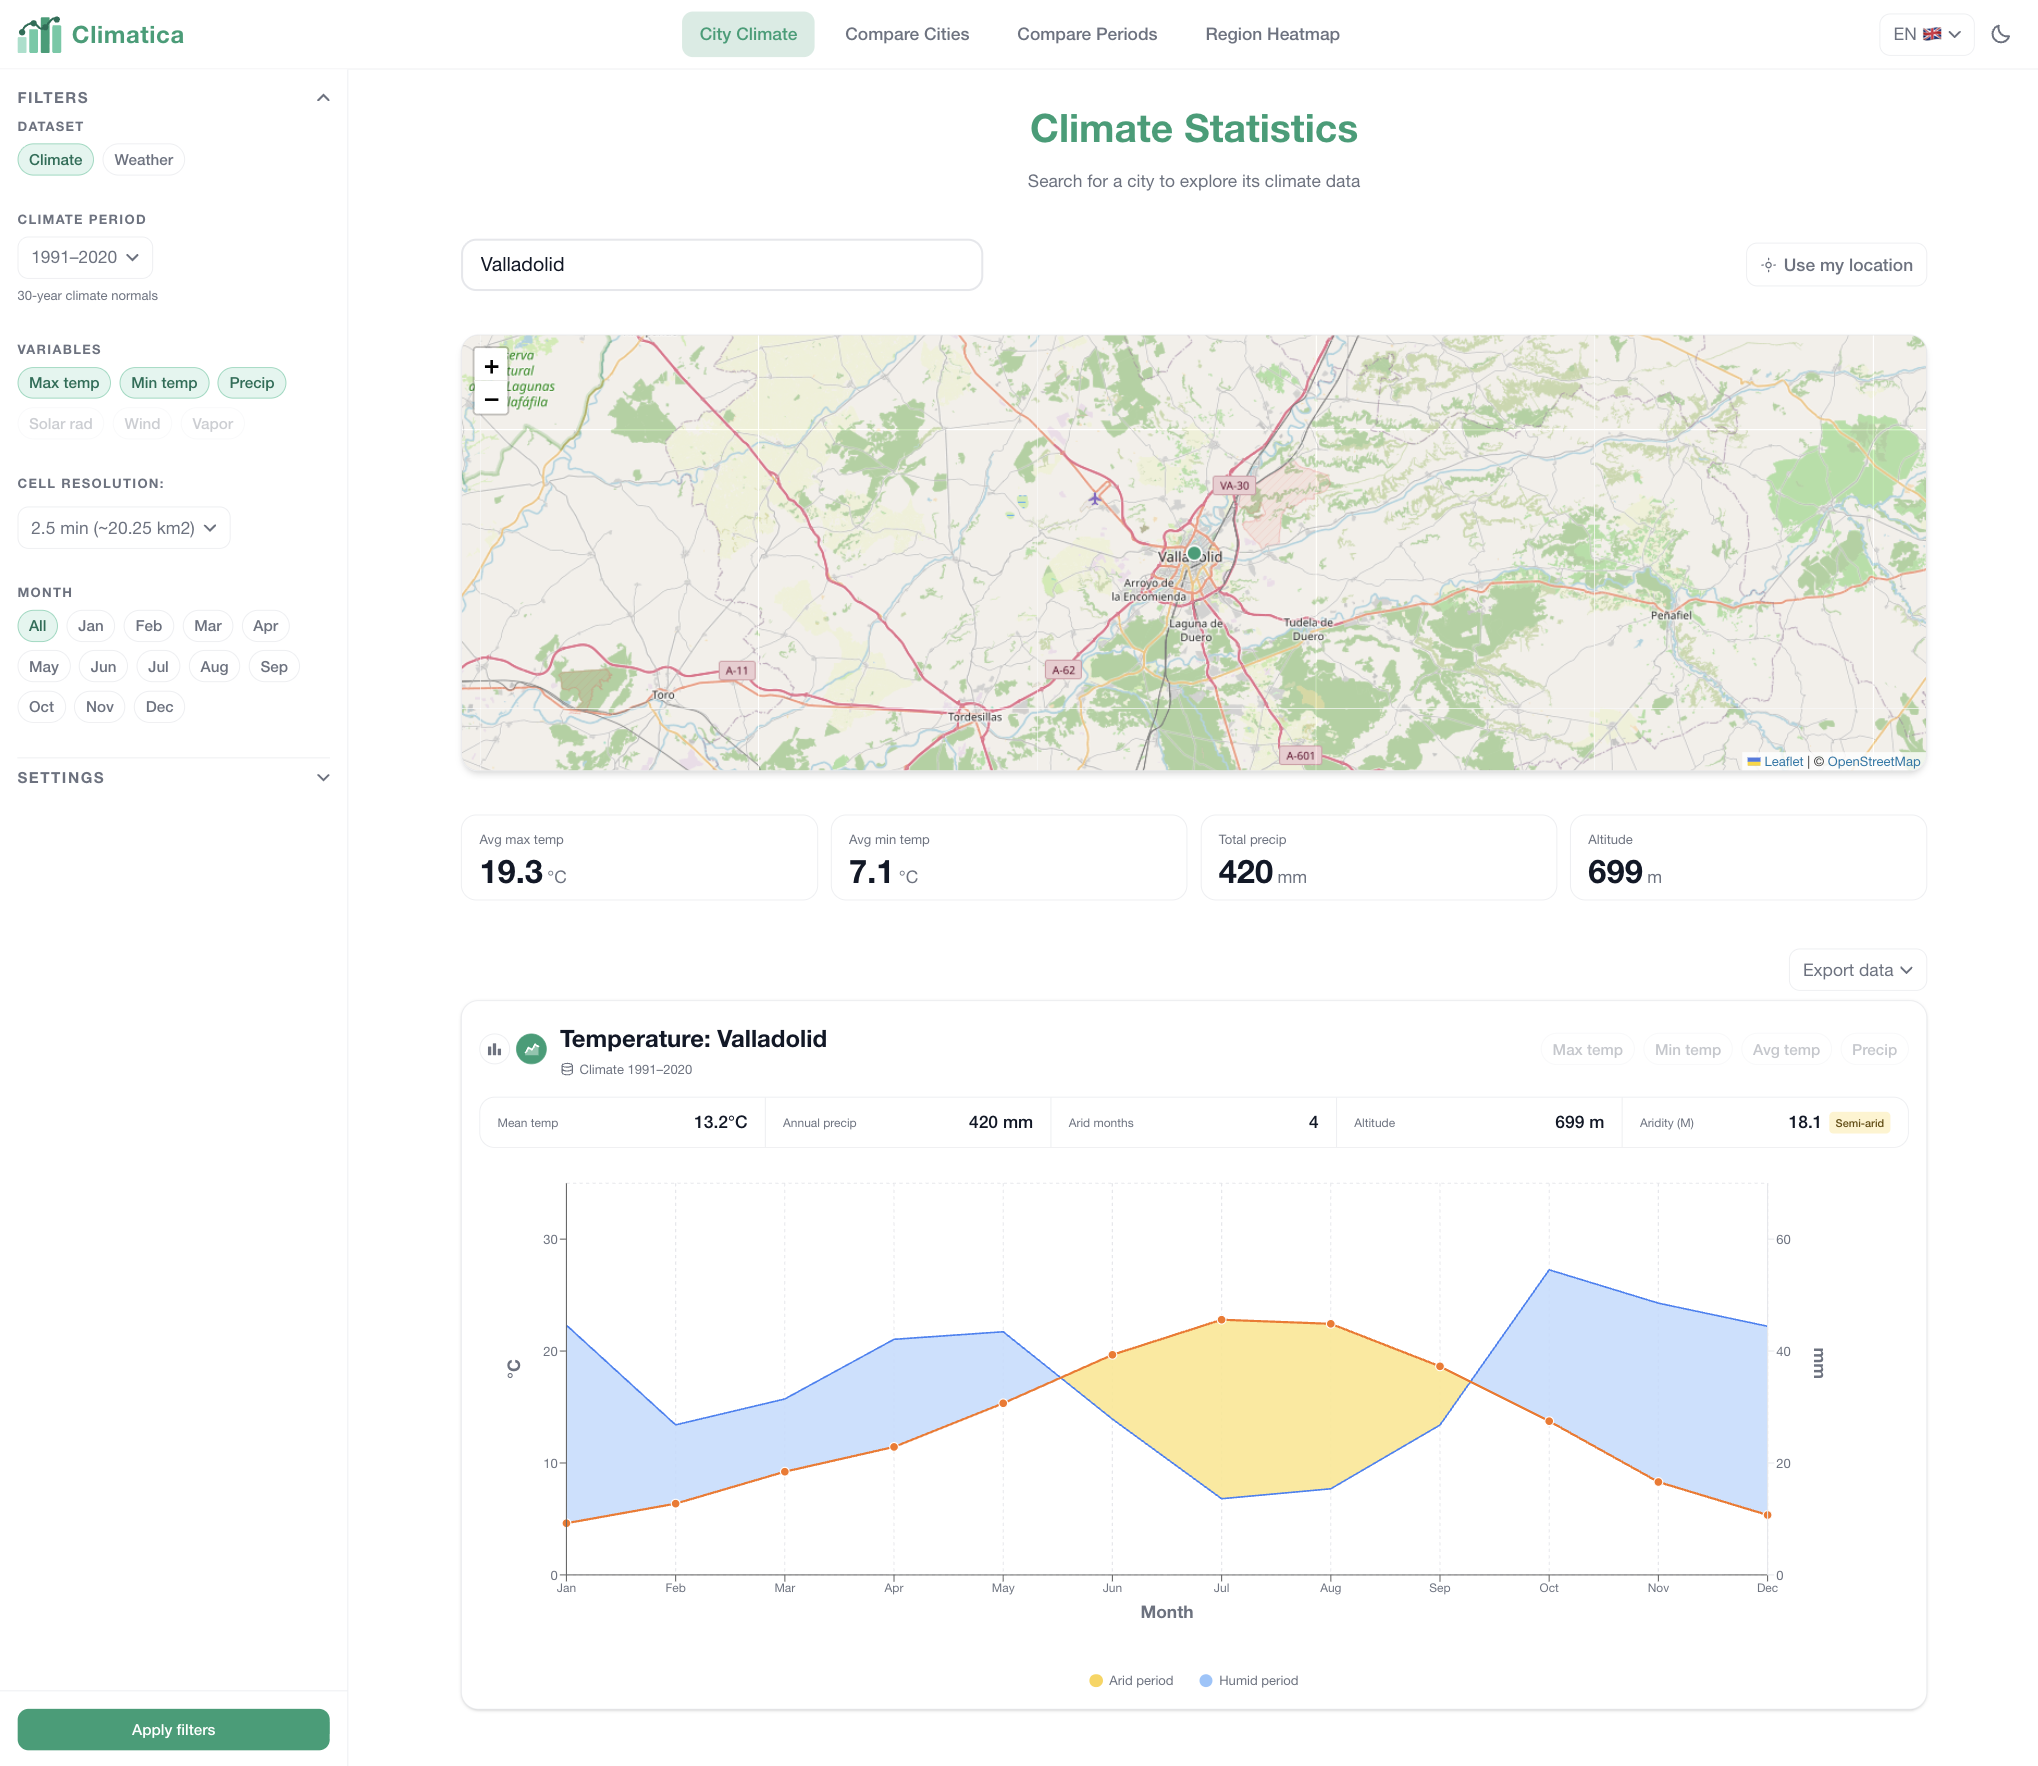
\includegraphics[width=\textwidth]{Images/climatica-demo-fmp-city-climate.png}
  \caption{City Climate page for Valladolid (climate dataset, 1991--2020
  normal). The Walter-Lieth climatogram shows four arid summer months
  (yellow area). The stat cards confirm an average maximum temperature of
  19.3\,$^\circ$C, total annual precipitation of 420\,mm, and a Martonne
  aridity index of 18.1 (Semi-arid).%
  \footnote{\url{https://climatica.gsic.uva.es/climate-statistics?city=Valladolid&lat=41.6554&lng=-4.7235&dataset=climate&var=tmax%2Ctmin%2Cprec&grid=5m&months=all&period=c1991-2020}}}
  
  \label{fig:demo_fmp_city}
\end{figure}

\subsubsection{Step 2: Detecting the Climate Shift}

The manager switches to the \textbf{Compare Periods} page and selects
Valladolid with the Climate dataset, setting Period~A to 1961--1990 and
Period~B to 1991--2020 (Figure~\ref{fig:demo_fmp_periods}). The statistics
table and overlaid chart immediately reveal the direction and magnitude of
the change: average maximum temperature increased by \textbf{+1.0\,$^\circ$C}
(from 18.3\,$^\circ$C to 19.3\,$^\circ$C), average minimum temperature
increased by +0.6\,$^\circ$C, and total annual precipitation decreased by
\textbf{11\,mm} (from 431\,mm to 420\,mm). The number of arid months
increased from 3 to 4 between the two periods, meaning that one additional 
month crossed the aridity threshold in the more recent normal. The Martonne 
aridity index dropped from 19.3 to 18.1, remaining in the Semi-arid category 
but moving further from the boundary with the less arid class.

The manager
records these figures in the FMP as evidence of an ongoing warming and drying
trend consistent with regional climate projections.

\begin{figure}[t]
  \centering
  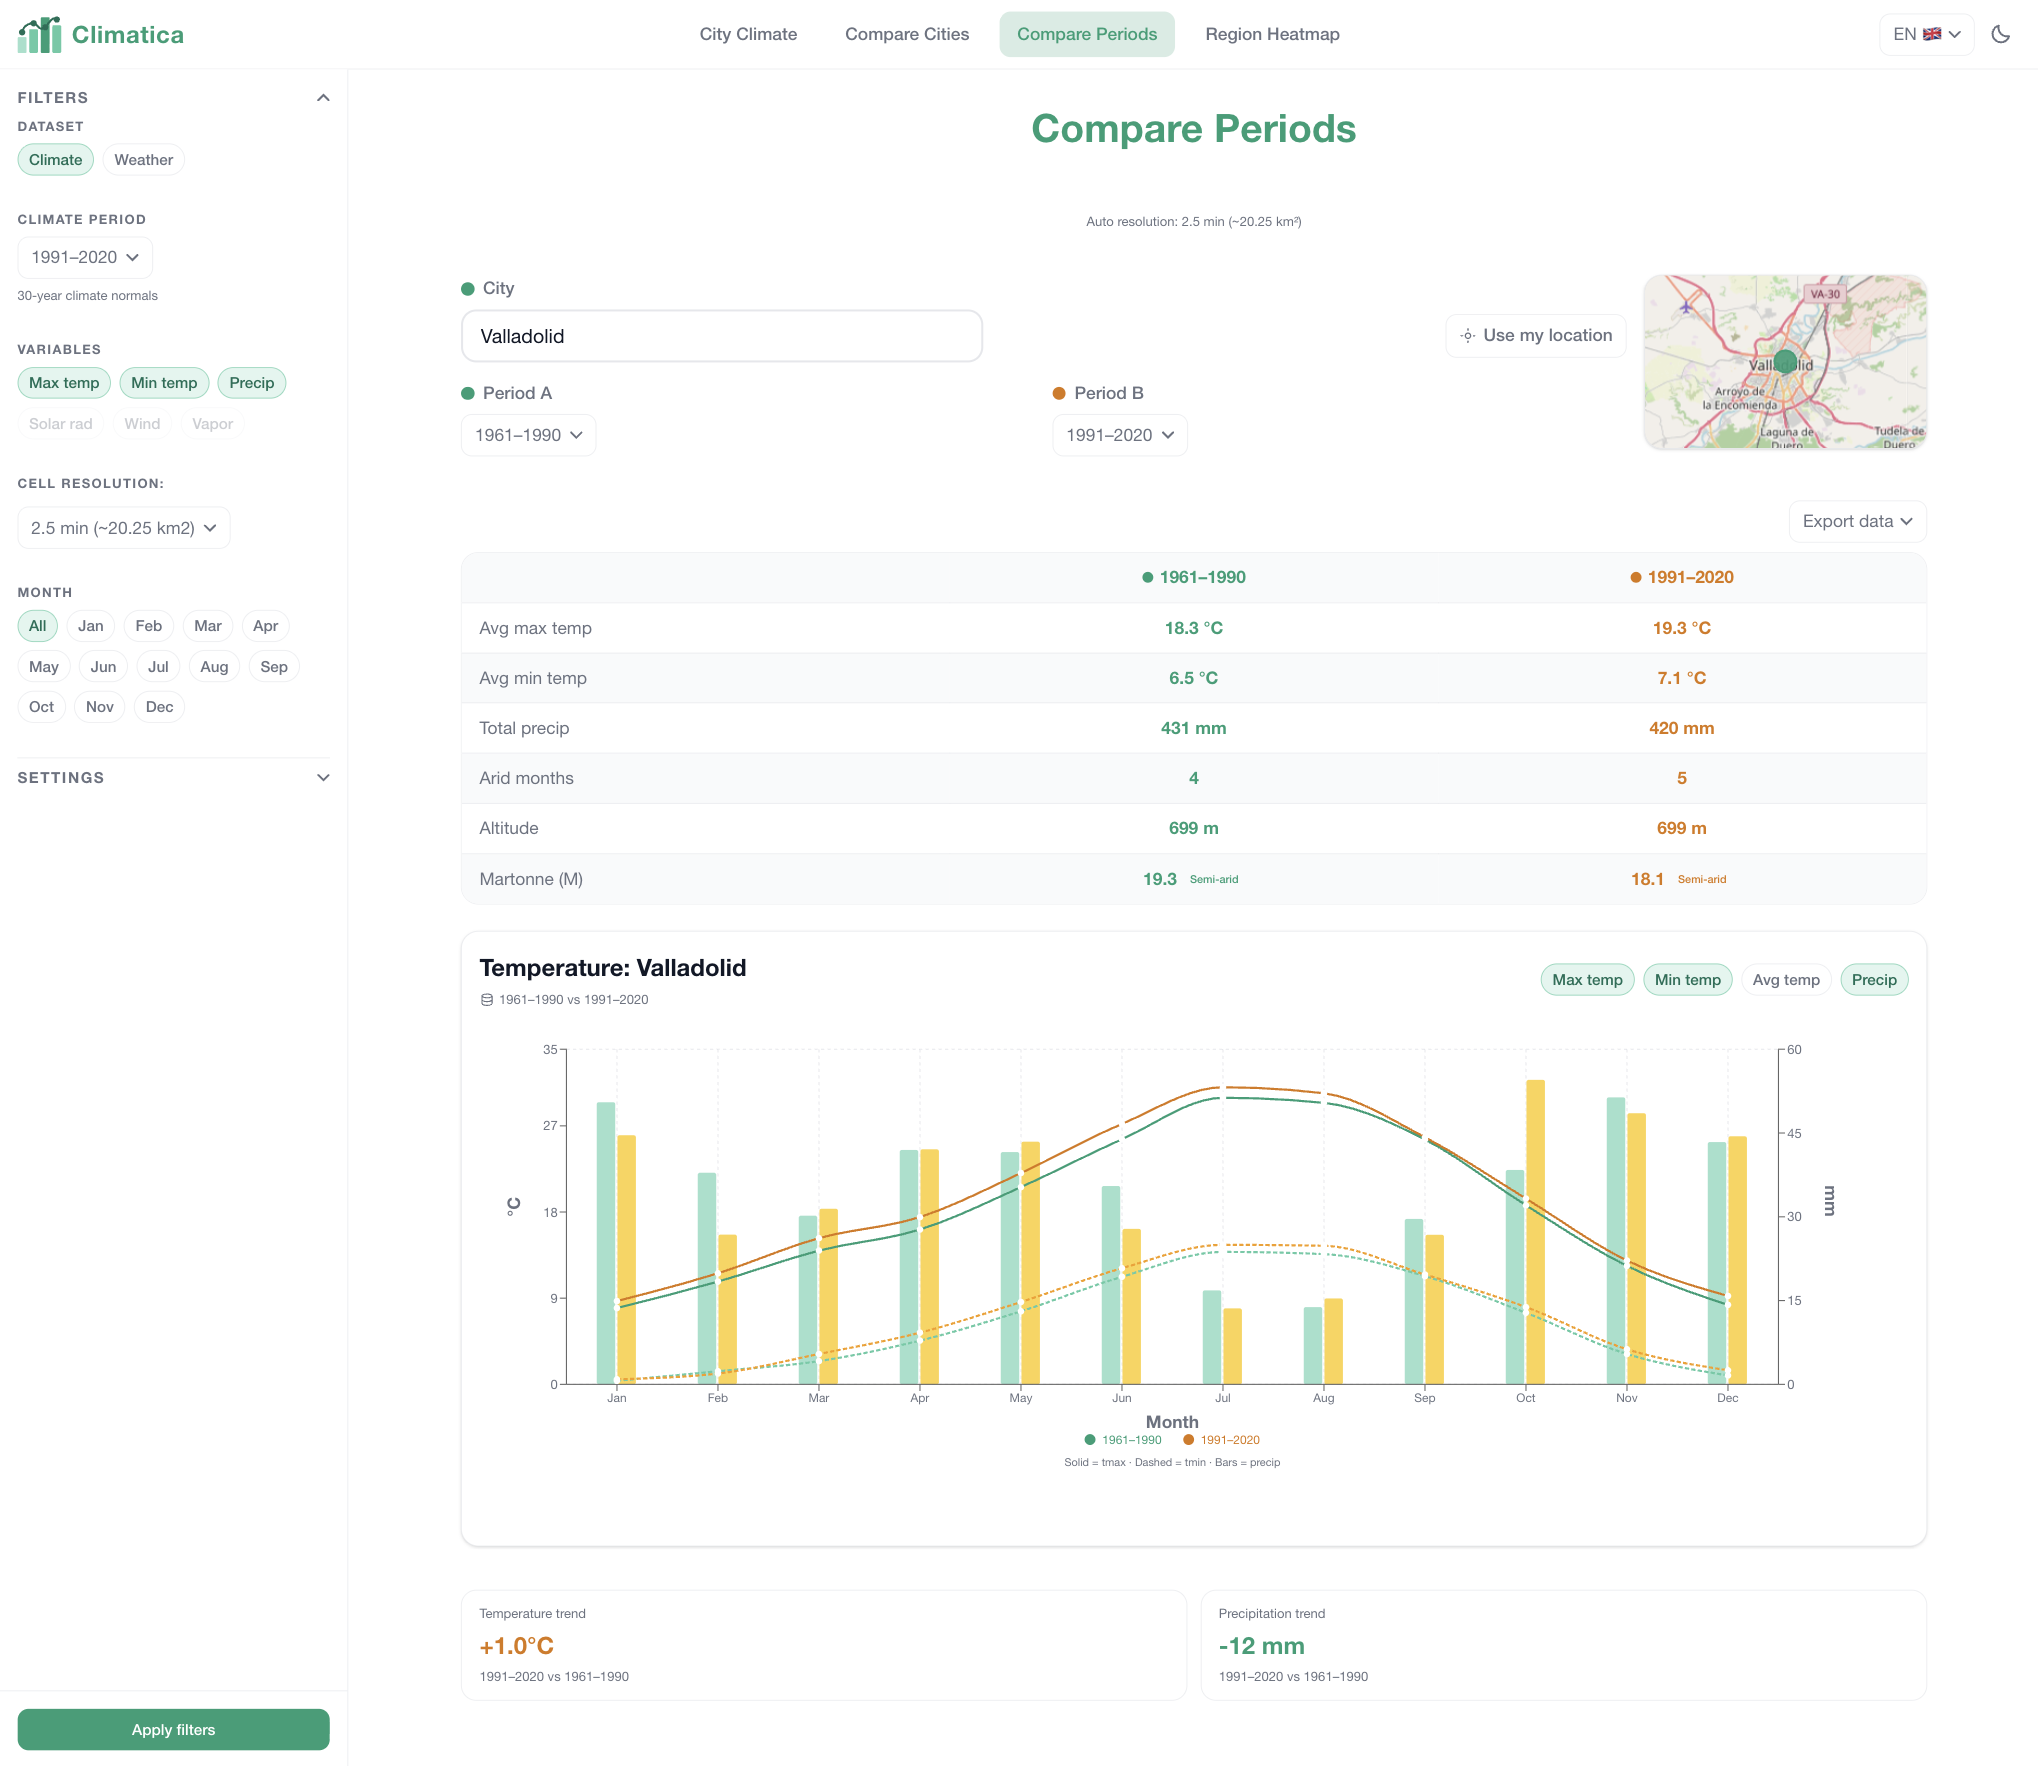
\includegraphics[width=\textwidth]{Images/climatica-demo-fmp-compare-periods.png}
  \caption{Compare Periods page for Valladolid comparing the 1961--1990 and
    1991--2020 climate normals. The statistics table shows a +1.0\,$^\circ$C
    increase in average maximum temperature and a decrease of 11\,mm in total
    precipitation. The trend indicator cards at the bottom confirm a
    temperature increase of +1.0\,$^\circ$C and a precipitation decrease of
    $-$12\,mm.%
    \footnote{\url{https://climatica.gsic.uva.es/compare-periods?city=Valladolid&lat=41.6554&lng=-4.7235&dataset=climate&var=tmax%2Ctmin%2Cprec&grid=5m&months=all&period1=c1961-1990&period2=c1991-2020}}}

  \label{fig:demo_fmp_periods}
\end{figure}

\subsubsection{Step 3: Spatial Distribution across the Management Unit}

Individual city data may not capture the full variability of a large management
unit. The manager switches to the \textbf{Region Heatmap} page, draws a
bounding box covering the area around Valladolid, and selects maximum
temperature under the 1991--2020 climate normal (Figure~\ref{fig:demo_fmp_heatmap}).
The resulting heatmap over 15 cells reveals a clear spatial gradient: the
urban core of Valladolid and the surrounding valley floor show the warmest
values (up to 17.7\,$^\circ$C annual average maximum), while the outlying
rural cells to the south and east are cooler (down to 15.1\,$^\circ$C). The
regional profile panel below the map confirms a mean temperature of
12.8\,$^\circ$C, annual precipitation of 425\,mm, and a Martonne index of
18.6 across the 15 queried cells.

This spatial resolution is directly actionable: stands in the warmer valley
cells are operating closer to thermal stress thresholds, while those in the
cooler peripheral cells have additional buffer. Species selection criteria may
legitimately differ between these sub-zones within the same management unit.

\begin{figure}[t]
  \centering
  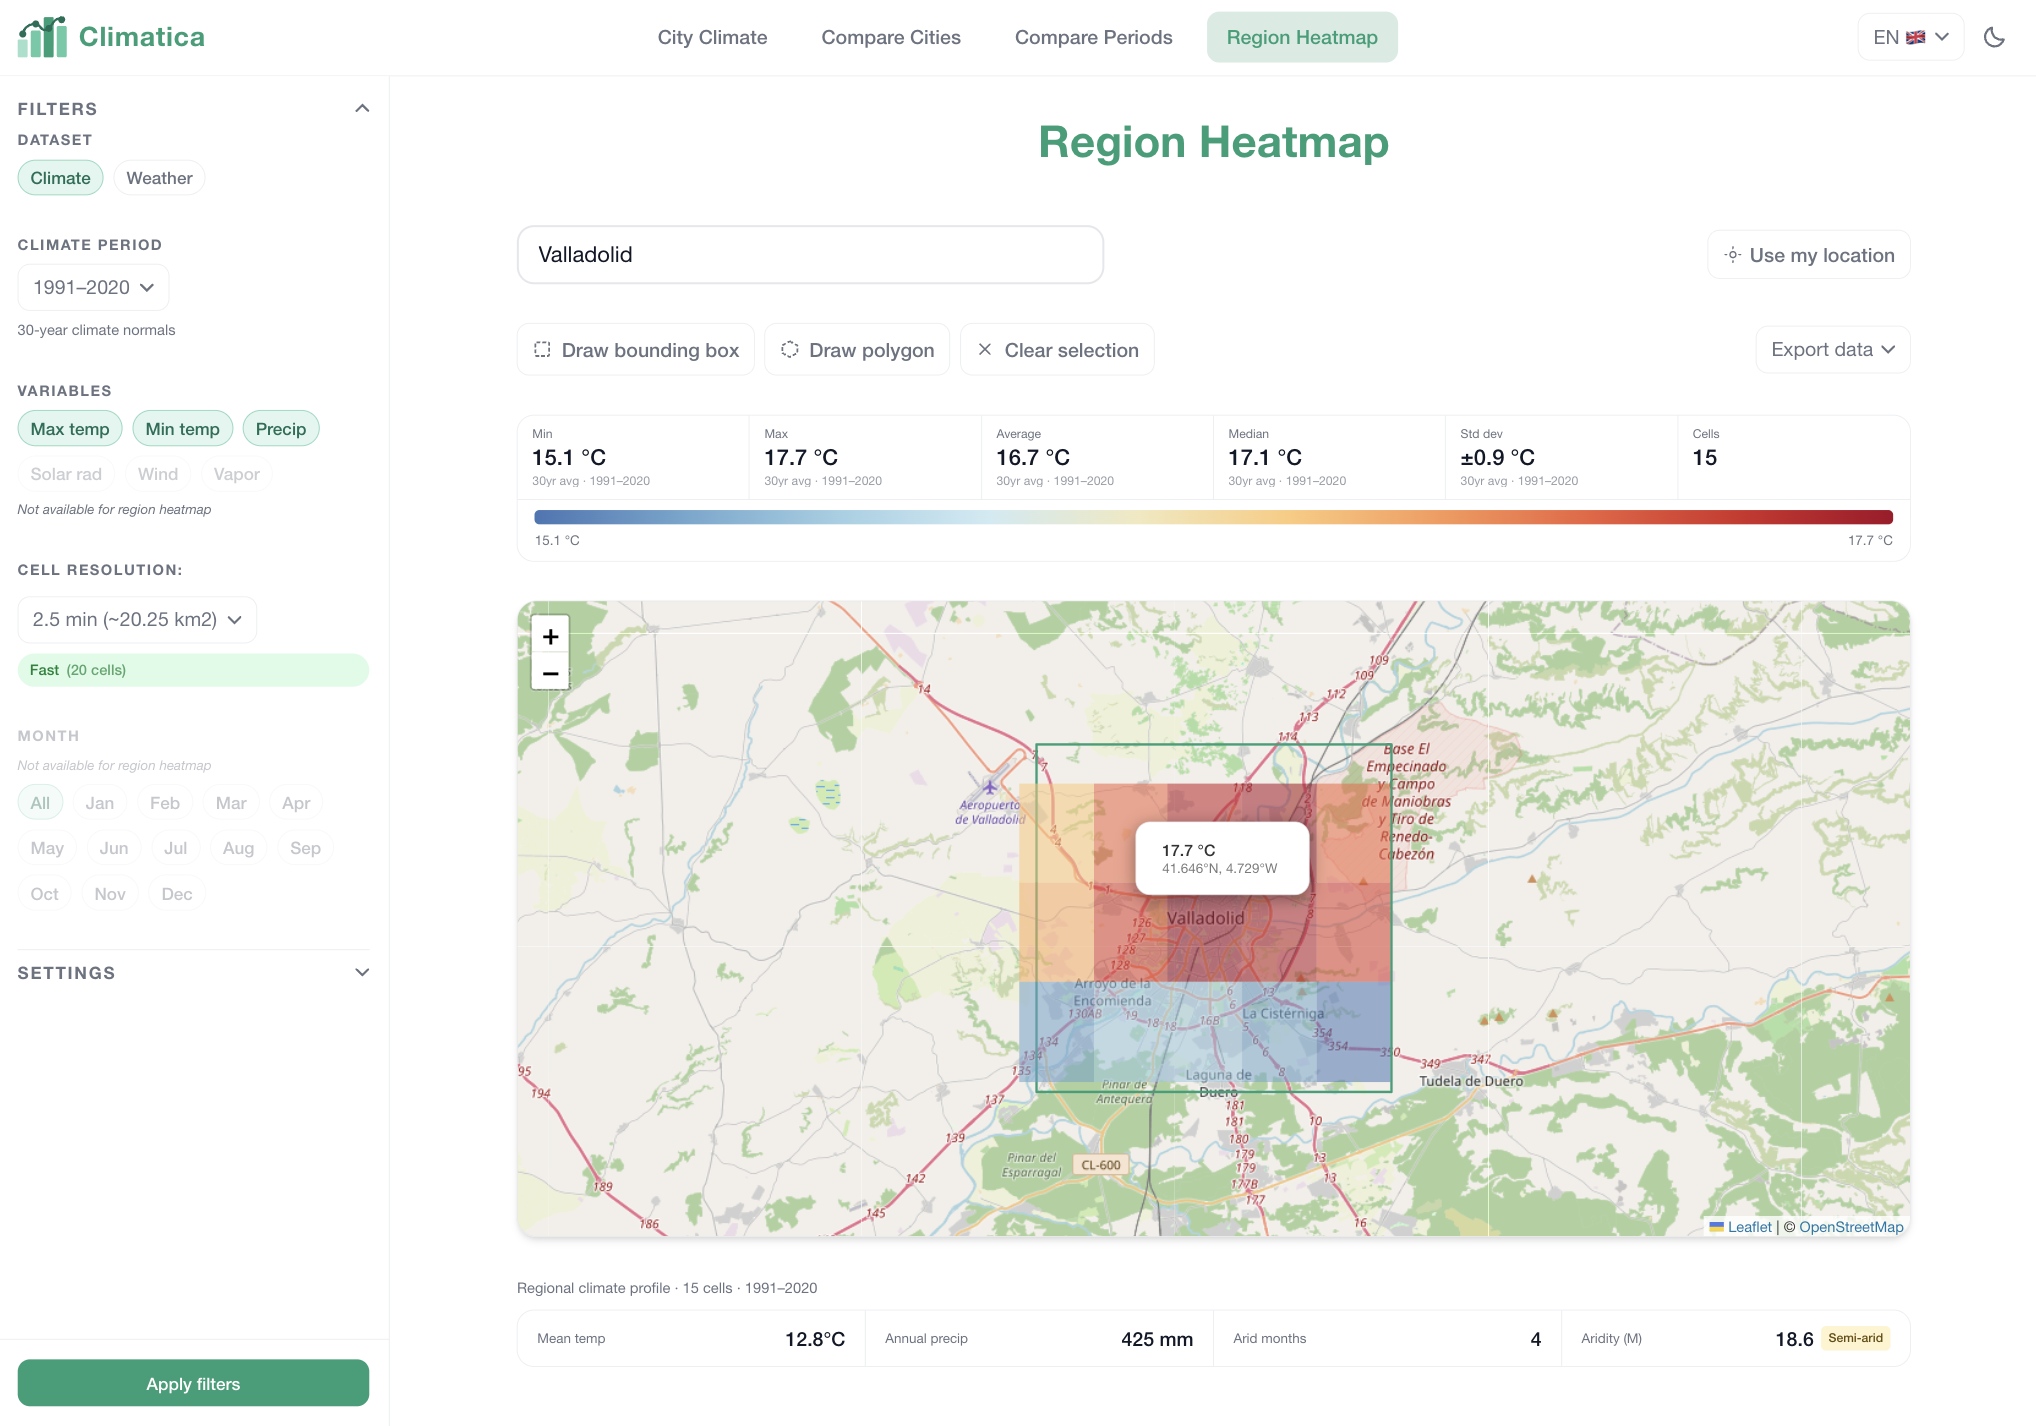
\includegraphics[width=\textwidth]{Images/climatica-demo-fmp-heatmap.png}
  \caption{Region Heatmap page showing the spatial distribution of annual
    average maximum temperature around Valladolid (climate dataset,
    1991--2020). The urban core reaches 17.7\,$^\circ$C while peripheral
    cells are as cool as 15.1\,$^\circ$C. The regional profile below the
    map summarises the 15 queried cells.%
    \footnote{\url{https://climatica.gsic.uva.es/heat-map?dataset=climate&var=tmax%2Ctmin%2Cprec&grid=2.5m&period=c1991-2020&north=41.723627485269766&south=41.58970039344626&west=-4.827399740322792&east=-4.643331682943493}}}

  \label{fig:demo_fmp_heatmap}
\end{figure}

\subsubsection{Step 4: Comparing Alternative Sites}

As a final step, the manager uses the \textbf{Compare Cities} page to place
Valladolid alongside \textbf{Salamanca}, a city 120\,km to the southwest
(Figure~\ref{fig:demo_fmp_cities}). The side-by-side comparison under the
1991--2020 normal shows that Salamanca is already warmer (+1.1\,$^\circ$C
average maximum), with both cities
sharing four arid months and a Martonne index in the Semi-arid range
(16.8 vs.\ 18.1). The insight cards at the bottom confirm that Salamanca is
the warmer city by 1.2\,$^\circ$C. The manager uses this comparison to inform
a precautionary approach: species that are currently performing well in
Salamanca's stands under equivalent soil conditions (\textit{Quercus suber},
\textit{Pinus pinaster}) are candidates for introduction into the Valladolid
management unit as climate analogues for mid-century conditions.

\begin{figure}[t]
  \centering
  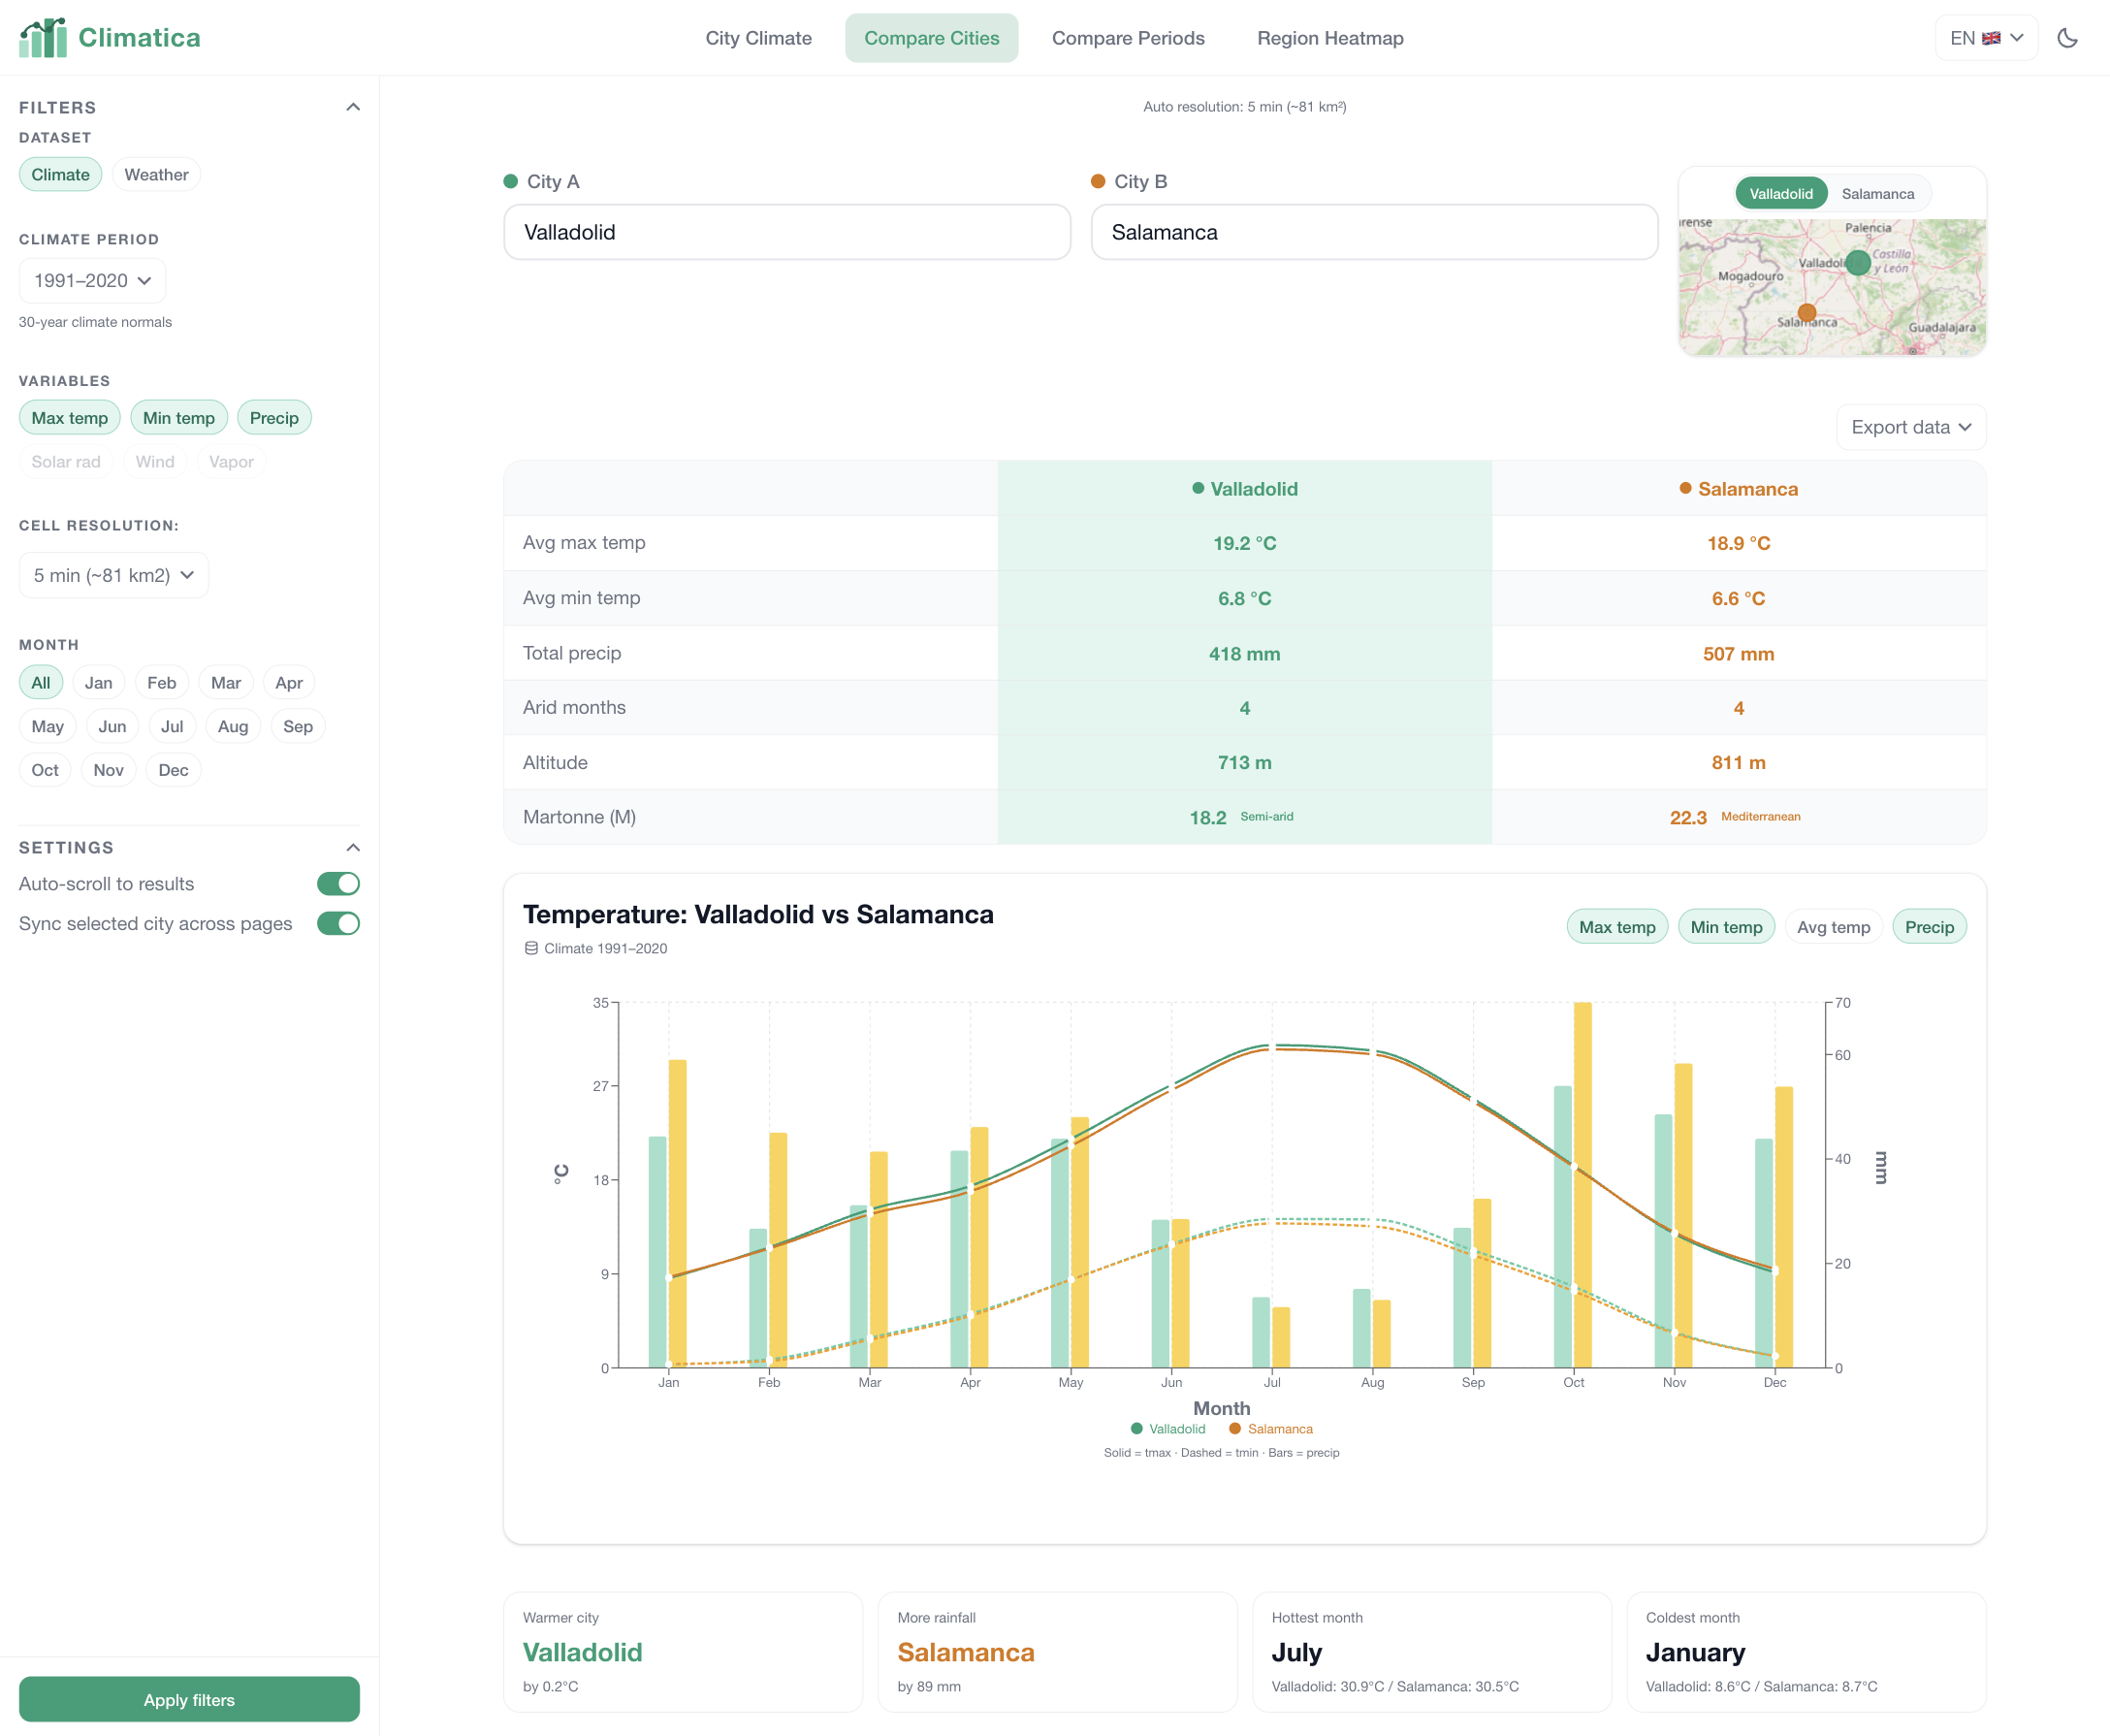
\includegraphics[width=\textwidth]{Images/climatica-demo-fmp-compare-cities.png}
  \caption{Compare Cities page placing Valladolid (green) alongside Salamanca
    (orange) under the 1991--2020 climate normal. Salamanca's higher average
    maximum temperature (20.4\,$^\circ$C vs.\ 19.3\,$^\circ$C) and lower
    Martonne index (16.8 vs.\ 18.1) make it a useful climate analogue for
    the conditions Valladolid may face in coming decades.%
    \footnote{\url{https://climatica.gsic.uva.es/compare-cities?cityA=Valladolid&latA=41.6554&lngA=-4.7235&cityB=Salamanca&latB=40.9688&lngB=-5.6639&dataset=climate&var=tmax%2Ctmin%2Cprec&grid=2.5m&period=c1991-2020}}}

  \label{fig:demo_fmp_cities}
\end{figure}

\subsubsection{Outcome}

In under fifteen minutes and without installing any software or writing any
code, the forest manager has: (1)~established the current climate baseline for
the site under the most recent 30-year normal; (2)~quantified the observed
shift over the past 60 years (+1.0\,$^\circ$C, $-$12\,mm, one additional arid
month); (3)~mapped the spatial variation in temperature across the management
unit at 2.5-minute resolution; and (4)~identified a nearby analogue site to
guide species selection under anticipated future conditions. All four pages of
Climatica contributed directly to this workflow, and the results are grounded
in the same WorldClim raster archive that would underpin a formal scientific
assessment.

\subsection{Scenario 2: Detecting Climate-Driven Forest Stress}\label{EVAL_DEMO_DECLINE}

\subsubsection{Context}

Climate change is increasingly recognised as a primary driver of forest decline
across Europe and North America. Warmer temperatures and prolonged summer
droughts weaken the physiological defences of trees, making them susceptible
to secondary agents --- most notably bark beetle outbreaks, which have caused
catastrophic mortality in spruce and pine stands across Central Europe and
Scandinavia over the past two decades~\cite{seidl2017bark}. Understanding
whether a particular site has experienced a meaningful shift towards warmer or
drier conditions over the period in which decline has been observed is a
necessary first step in attributing mortality to climate stress rather than to
other causes such as competition, soil degradation, or pathogen pressure.

An ecologist investigating pine stands in the western Pyrenees that have shown
elevated mortality and bark beetle damage since approximately 2010 wants to
establish whether the local climate has shifted meaningfully over the study
period. The nearest city representative of the study area is \textbf{Pamplona}
(Navarra, Spain).

\subsubsection{Step 1: Multi-period Temperature Trend}

The ecologist opens the \textbf{Compare Periods} page, selects Pamplona, and
switches to Weather mode. Using the multi-year selector in the sidebar, five
years are chosen to span the full observation window: 1985, 1995, 2005, 2015,
and 2023. Each year is assigned a distinct colour (green, amber, blue, rose,
violet) and the overlaid chart renders all five maximum temperature curves
simultaneously (Figure~\ref{fig:demo_decline_multiyear}).

The statistics table reveals a clear warming signal: average annual maximum
temperature increased from 17.7\,$^\circ$C in 1985 to 19.6\,$^\circ$C in
2023 --- a rise of \textbf{+1.9\,$^\circ$C} over 38 years. The year 2015
stands out with the highest average maximum temperature (18.7\,$^\circ$C),
consistent with the record European heat conditions of that year~\cite{ipcc2021}. The tooltip
on the July peak confirms that July maximum temperatures were 27\,$^\circ$C
in 1985--2005 and rose to 28--29\,$^\circ$C in 2015--2023.

\begin{figure}[t]
  \centering
  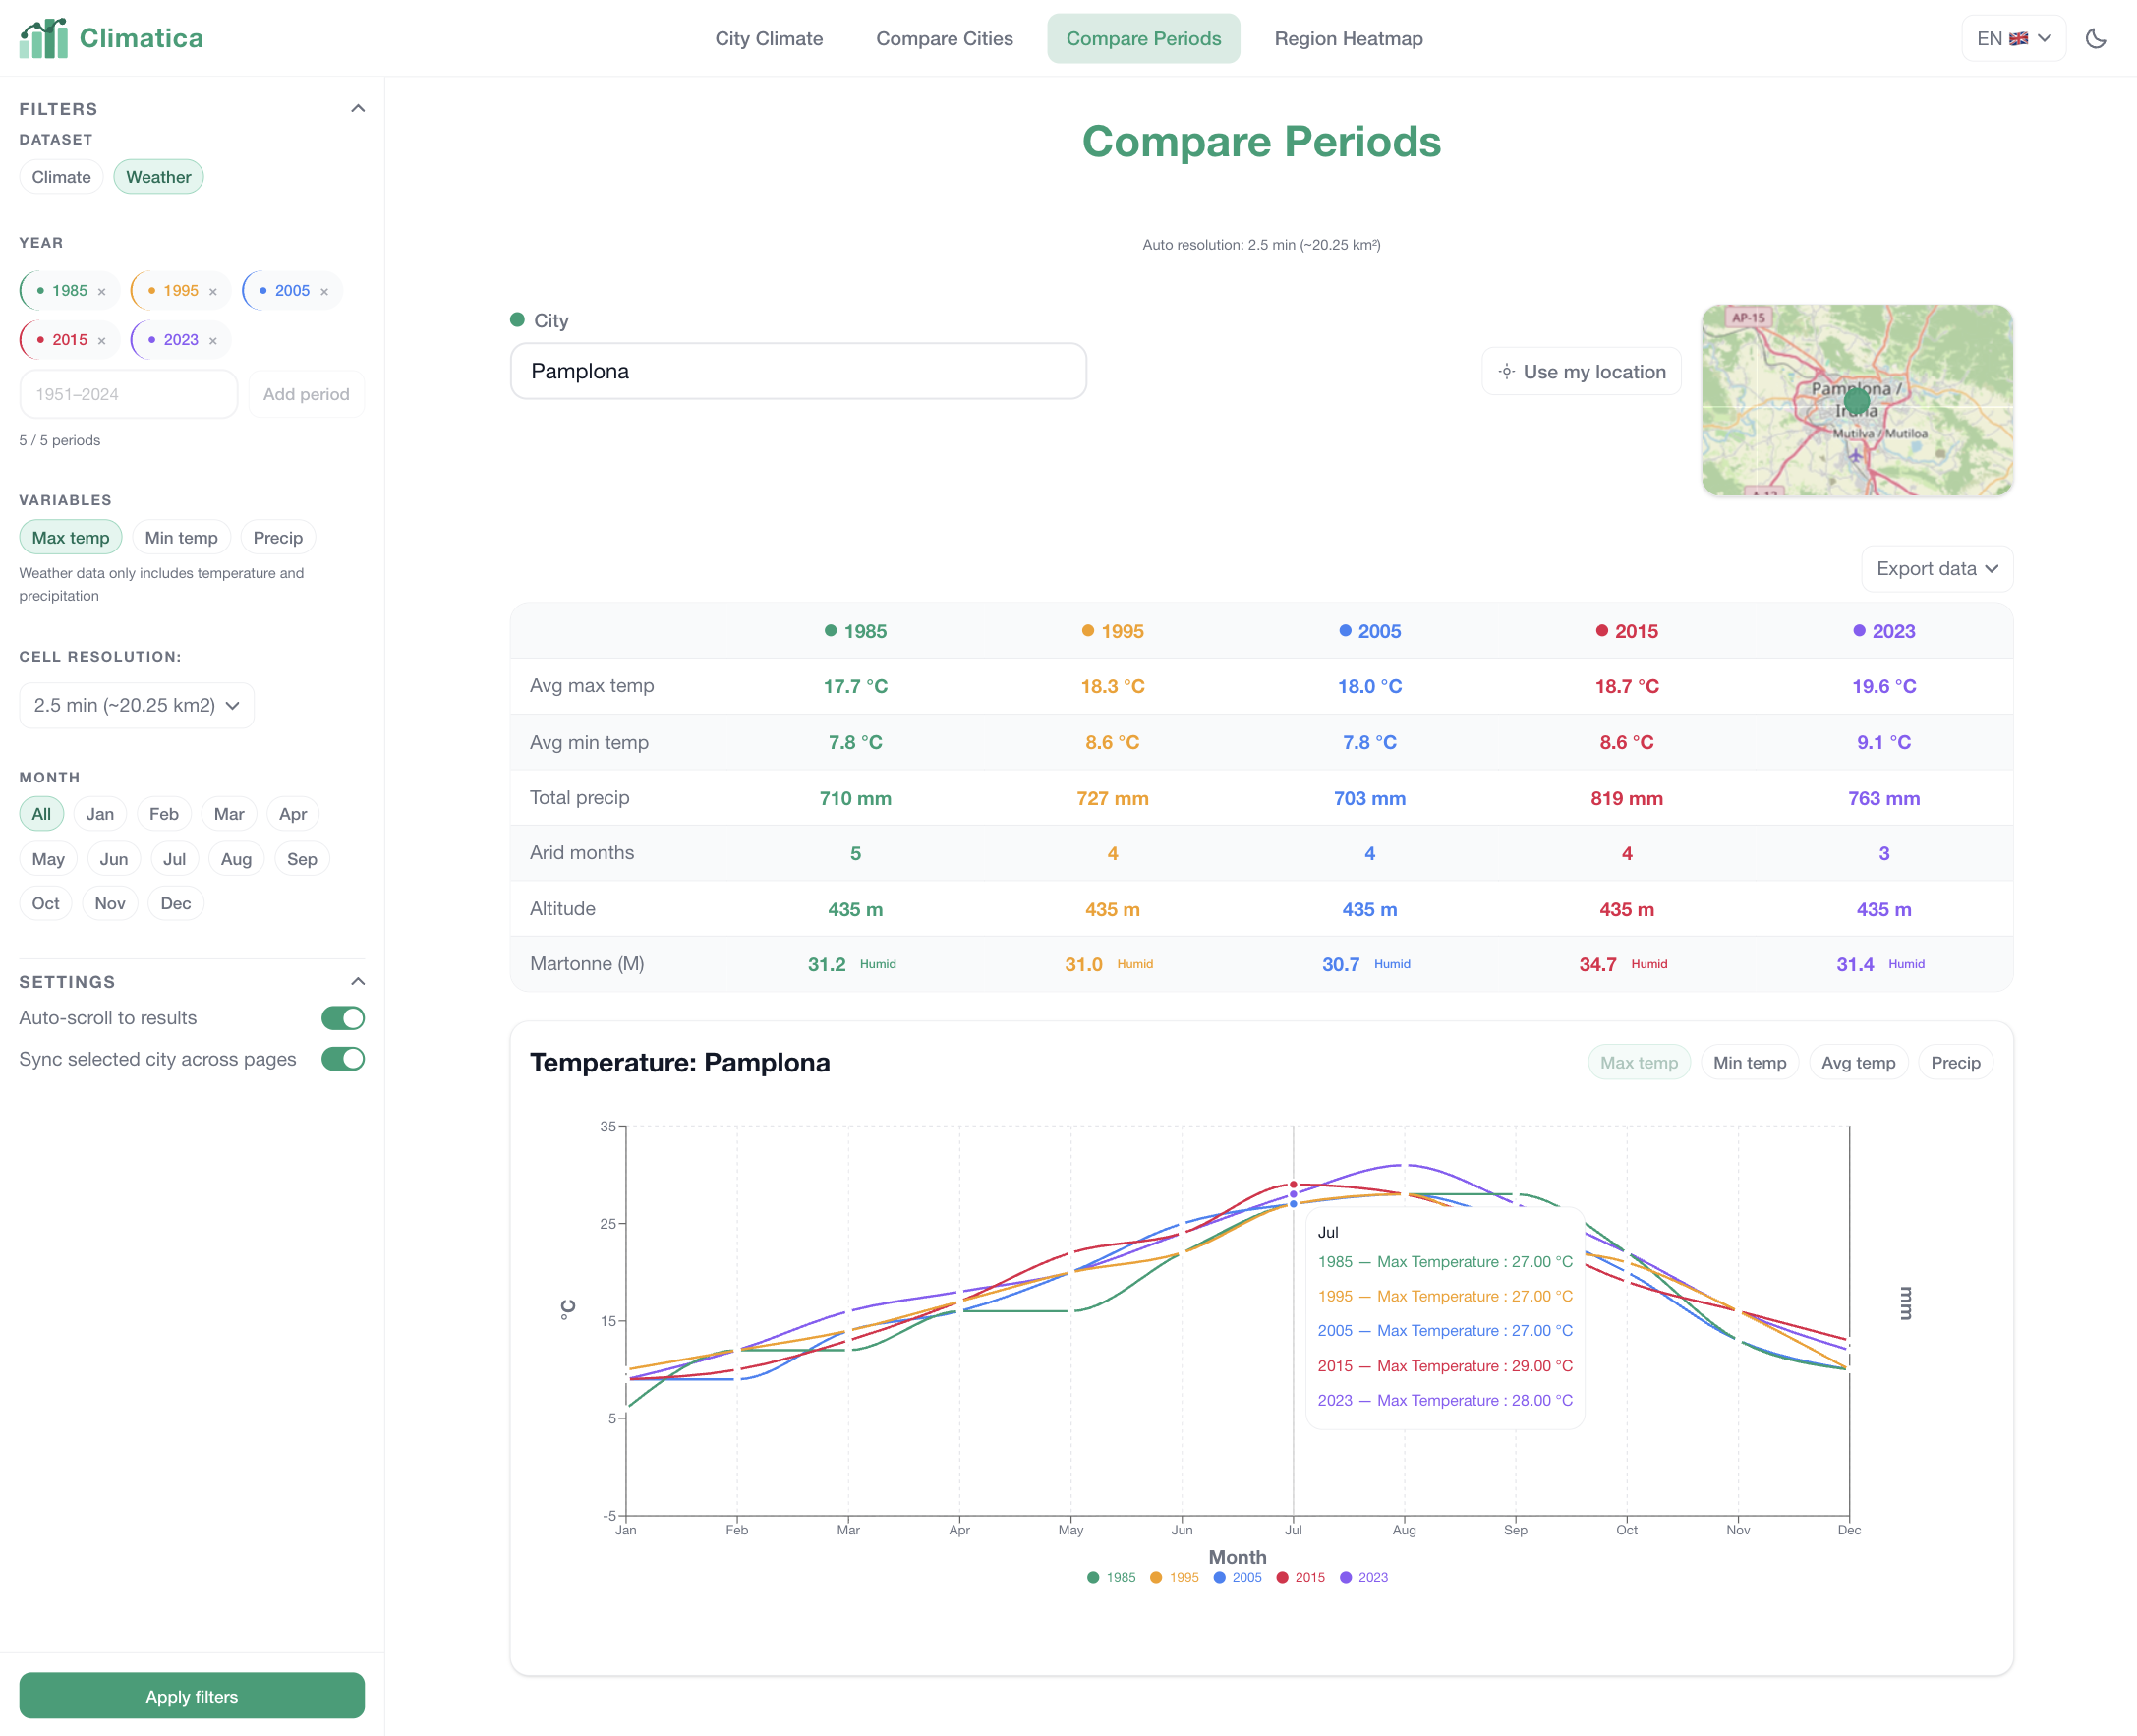
\includegraphics[width=\textwidth]{Images/climatica-demo-decline-multiyear.png}
  \caption{Compare Periods page in weather mode for Pamplona showing five
    selected years (1985, 1995, 2005, 2015, 2023) with maximum temperature.
    The statistics table shows average annual maximum temperature rising from
    17.7\,$^\circ$C in 1985 to 19.6\,$^\circ$C in 2023 (+1.9\,$^\circ$C).
    The tooltip confirms July maximum temperatures of 27\,$^\circ$C in the
    earlier years versus 28--29\,$^\circ$C in recent years.%
    \footnote{\url{https://climatica.gsic.uva.es/compare-periods?city=Pamplona&lat=42.8169&lng=-1.6432&dataset=weather&var=tmax%2Ctmin%2Cprec&grid=2.5m&months=all&periods=1985%2C1995%2C2005%2C2015%2C2023}}}

  \label{fig:demo_decline_multiyear}
\end{figure}

\subsubsection{Step 2: Precipitation and Aridity Trend}

The ecologist switches the chart variable to \textbf{Precipitation}
(Figure~\ref{fig:demo_decline_precip}). The picture here is more variable:
total annual precipitation ranges from 703\,mm (2005) to 819\,mm (2015),
with no clear monotonic trend. However, the Martonne aridity index in the
statistics table shows that all five years remain in the \emph{Humid} category
(M~$>$~30), with values between 30.7 and 34.7. The bar chart reveals that
inter-annual variability in summer precipitation is high, with some years
showing near-zero July and August precipitation while others show moderate
values. The combination of rising maximum temperatures and variable but
occasionally very dry summers creates the drought stress conditions most
damaging to \textit{Pinus sylvestris}.

\begin{figure}[t]
  \centering
  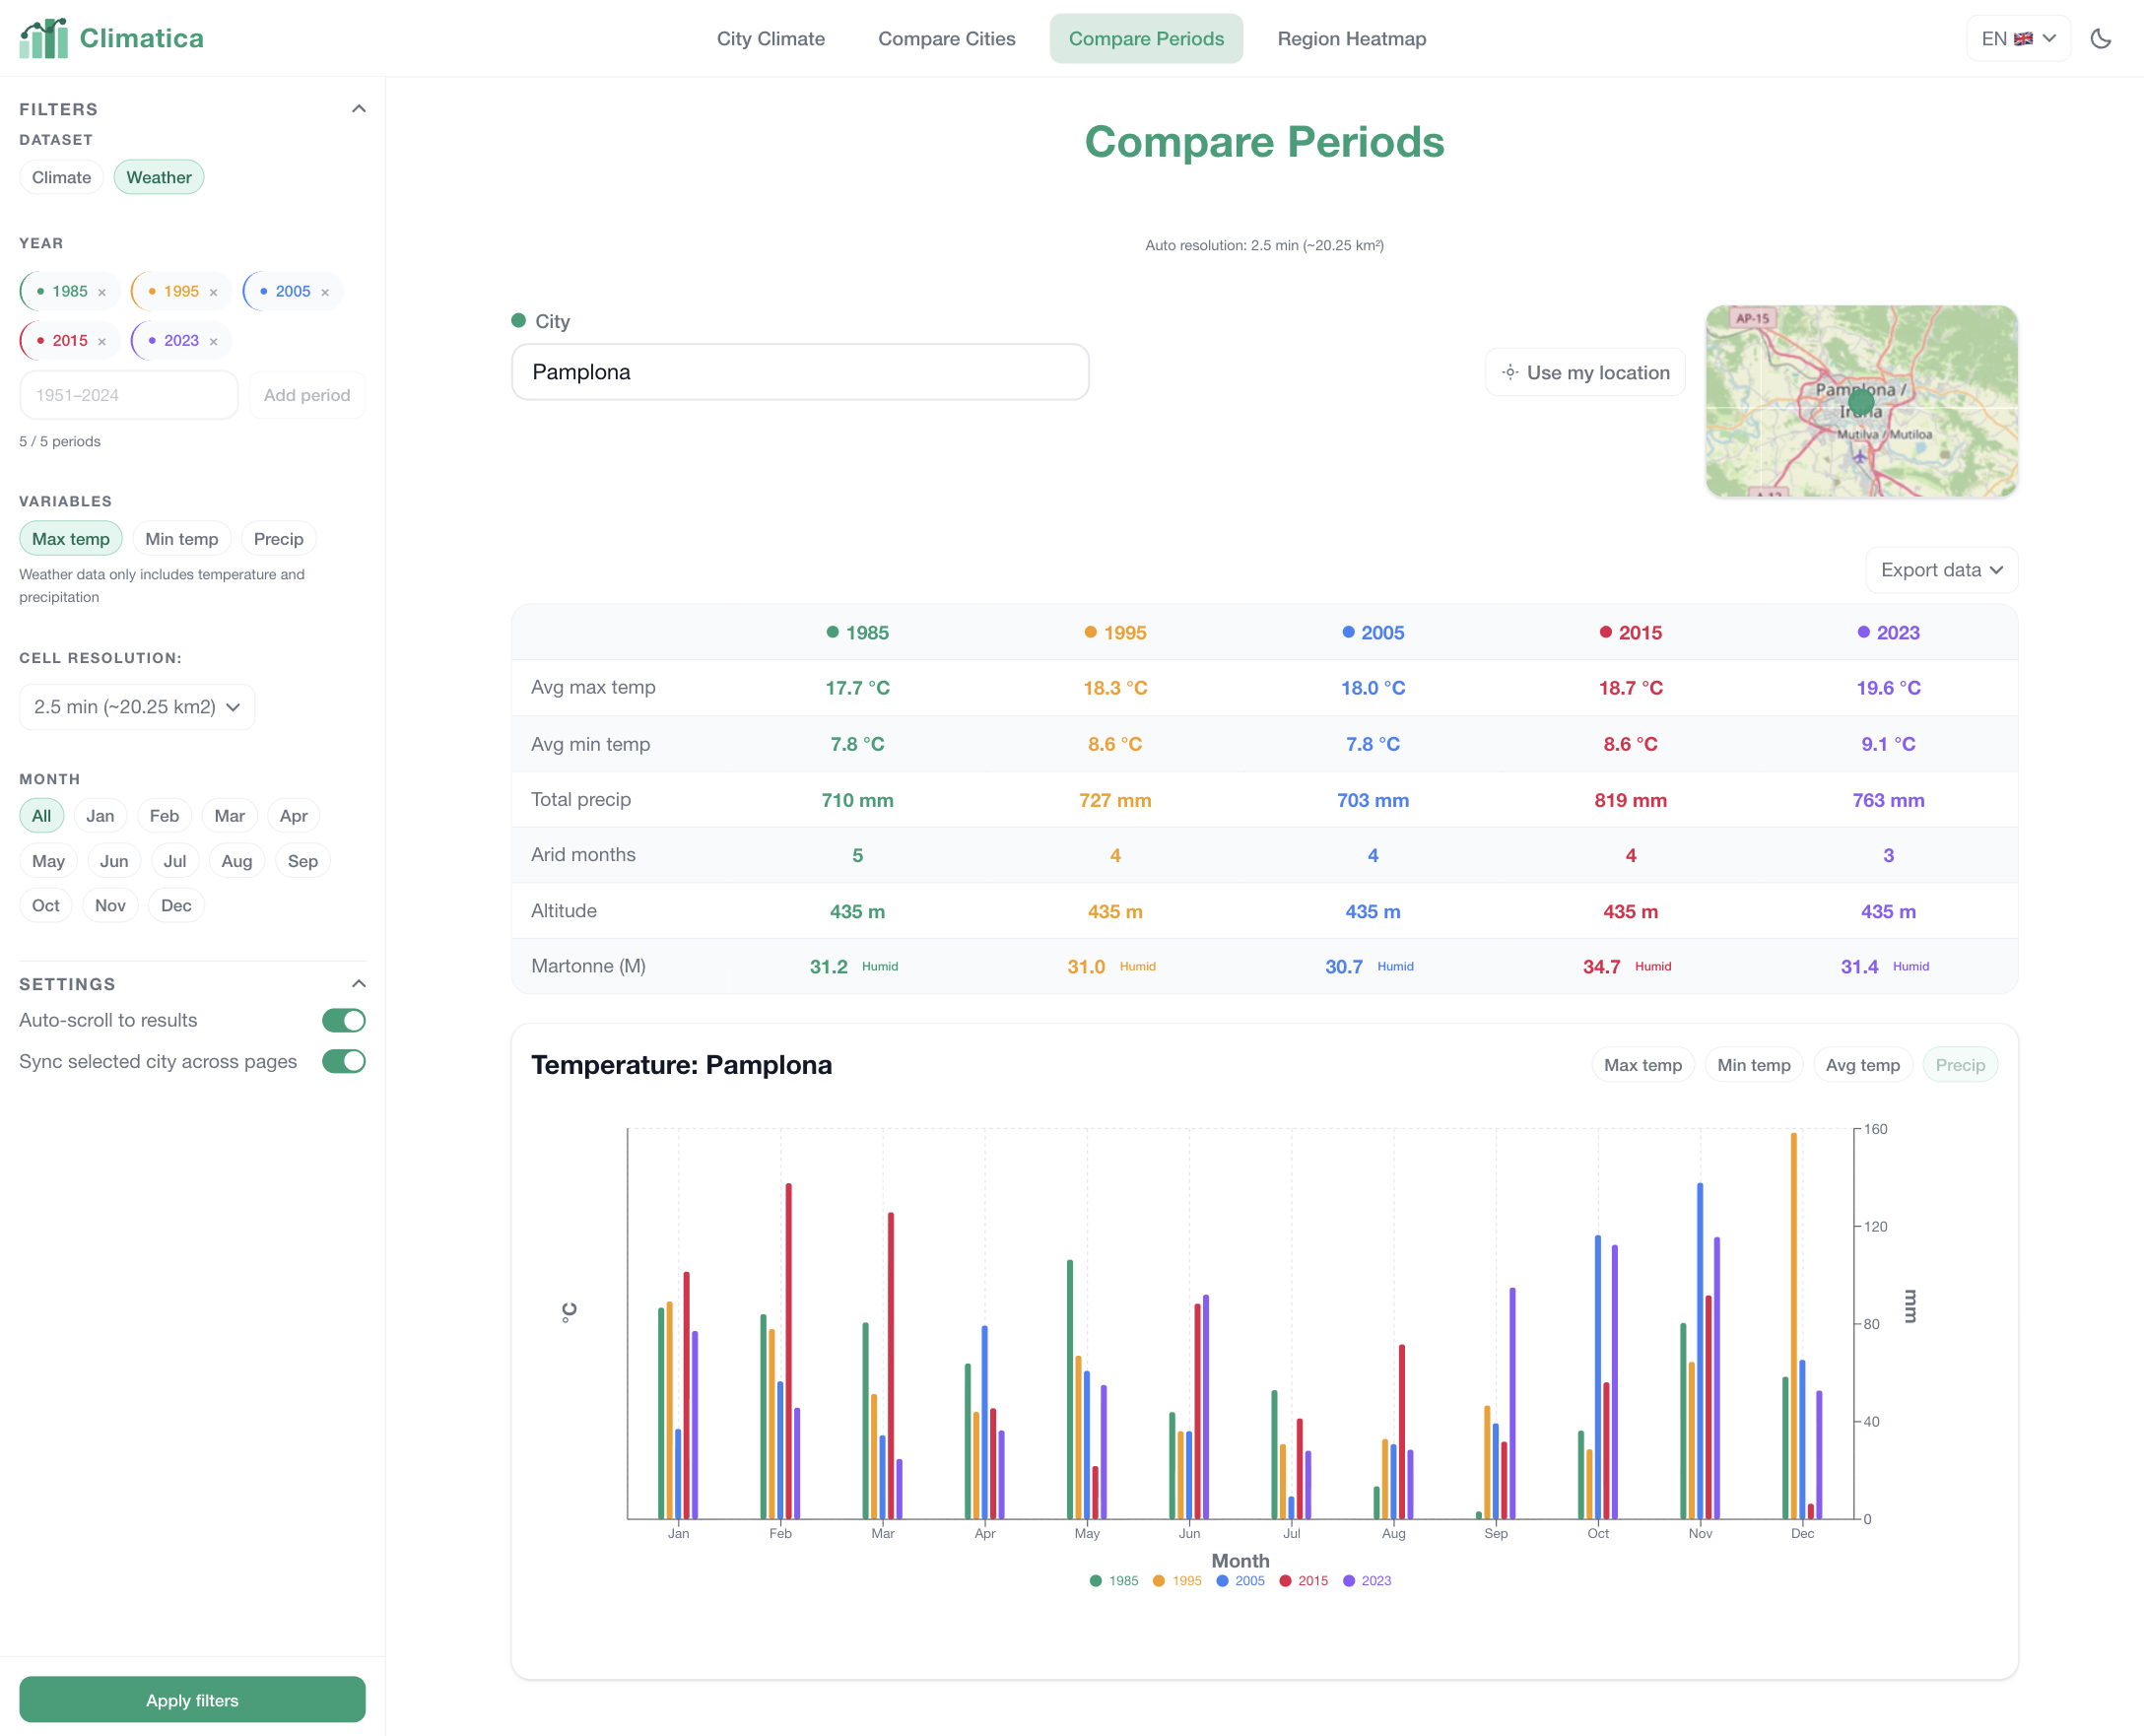
\includegraphics[width=\textwidth]{Images/climatica-demo-decline-precipitation.png}
  \caption{Compare Periods page in weather mode for Pamplona with precipitation
    selected. The bar chart shows high inter-annual variability in summer
    precipitation across the five years. The Martonne index (30.7--34.7)
    keeps all years in the Humid category, but the combination of rising
    temperatures and occasional summer drought creates physiological stress
    conditions for conifers.%
    \footnote{\url{https://climatica.gsic.uva.es/compare-periods?city=Pamplona&lat=42.8169&lng=-1.6432&dataset=weather&var=tmax%2Ctmin%2Cprec&grid=2.5m&months=all&periods=1985%2C1995%2C2005%2C2015%2C2023}}}

  \label{fig:demo_decline_precip}
\end{figure}

\subsubsection{Step 3: Spatial Extent of the Stress Signal}

To assess whether the stress conditions are localised or part of a broader
regional pattern, the ecologist switches to the \textbf{Region Heatmap} page
and draws a polygon around the Pyrenean foothills east of Pamplona
(Figure~\ref{fig:demo_decline_heatmap}). Using the weather dataset for 1991,
the heatmap over 34 cells reveals a strong elevation-driven thermal gradient:
the lowland cells in the Ebro valley to the south reach annual average maximum
temperatures above 11\,$^\circ$C, while the higher-elevation cells in the
Pyrenean ranges to the north are distinctly cooler (down to 6.8\,$^\circ$C).
The regional profile confirms a mean temperature of 11.0\,$^\circ$C, annual
precipitation of 918\,mm, and a Martonne index of 43.8 (\emph{Very-humid}) ---
conditions that support dense conifer forest but that are increasingly
susceptible to drought stress during anomalously dry summers.

The spatial pattern makes clear that the bark beetle risk is not uniform across
the landscape: the warmer, south-facing lowland cells are under greater thermal
stress than the cooler highland cells, and any management intervention aimed
at reducing stand vulnerability should prioritise the lower-elevation zones.

\begin{figure}[t]
  \centering
  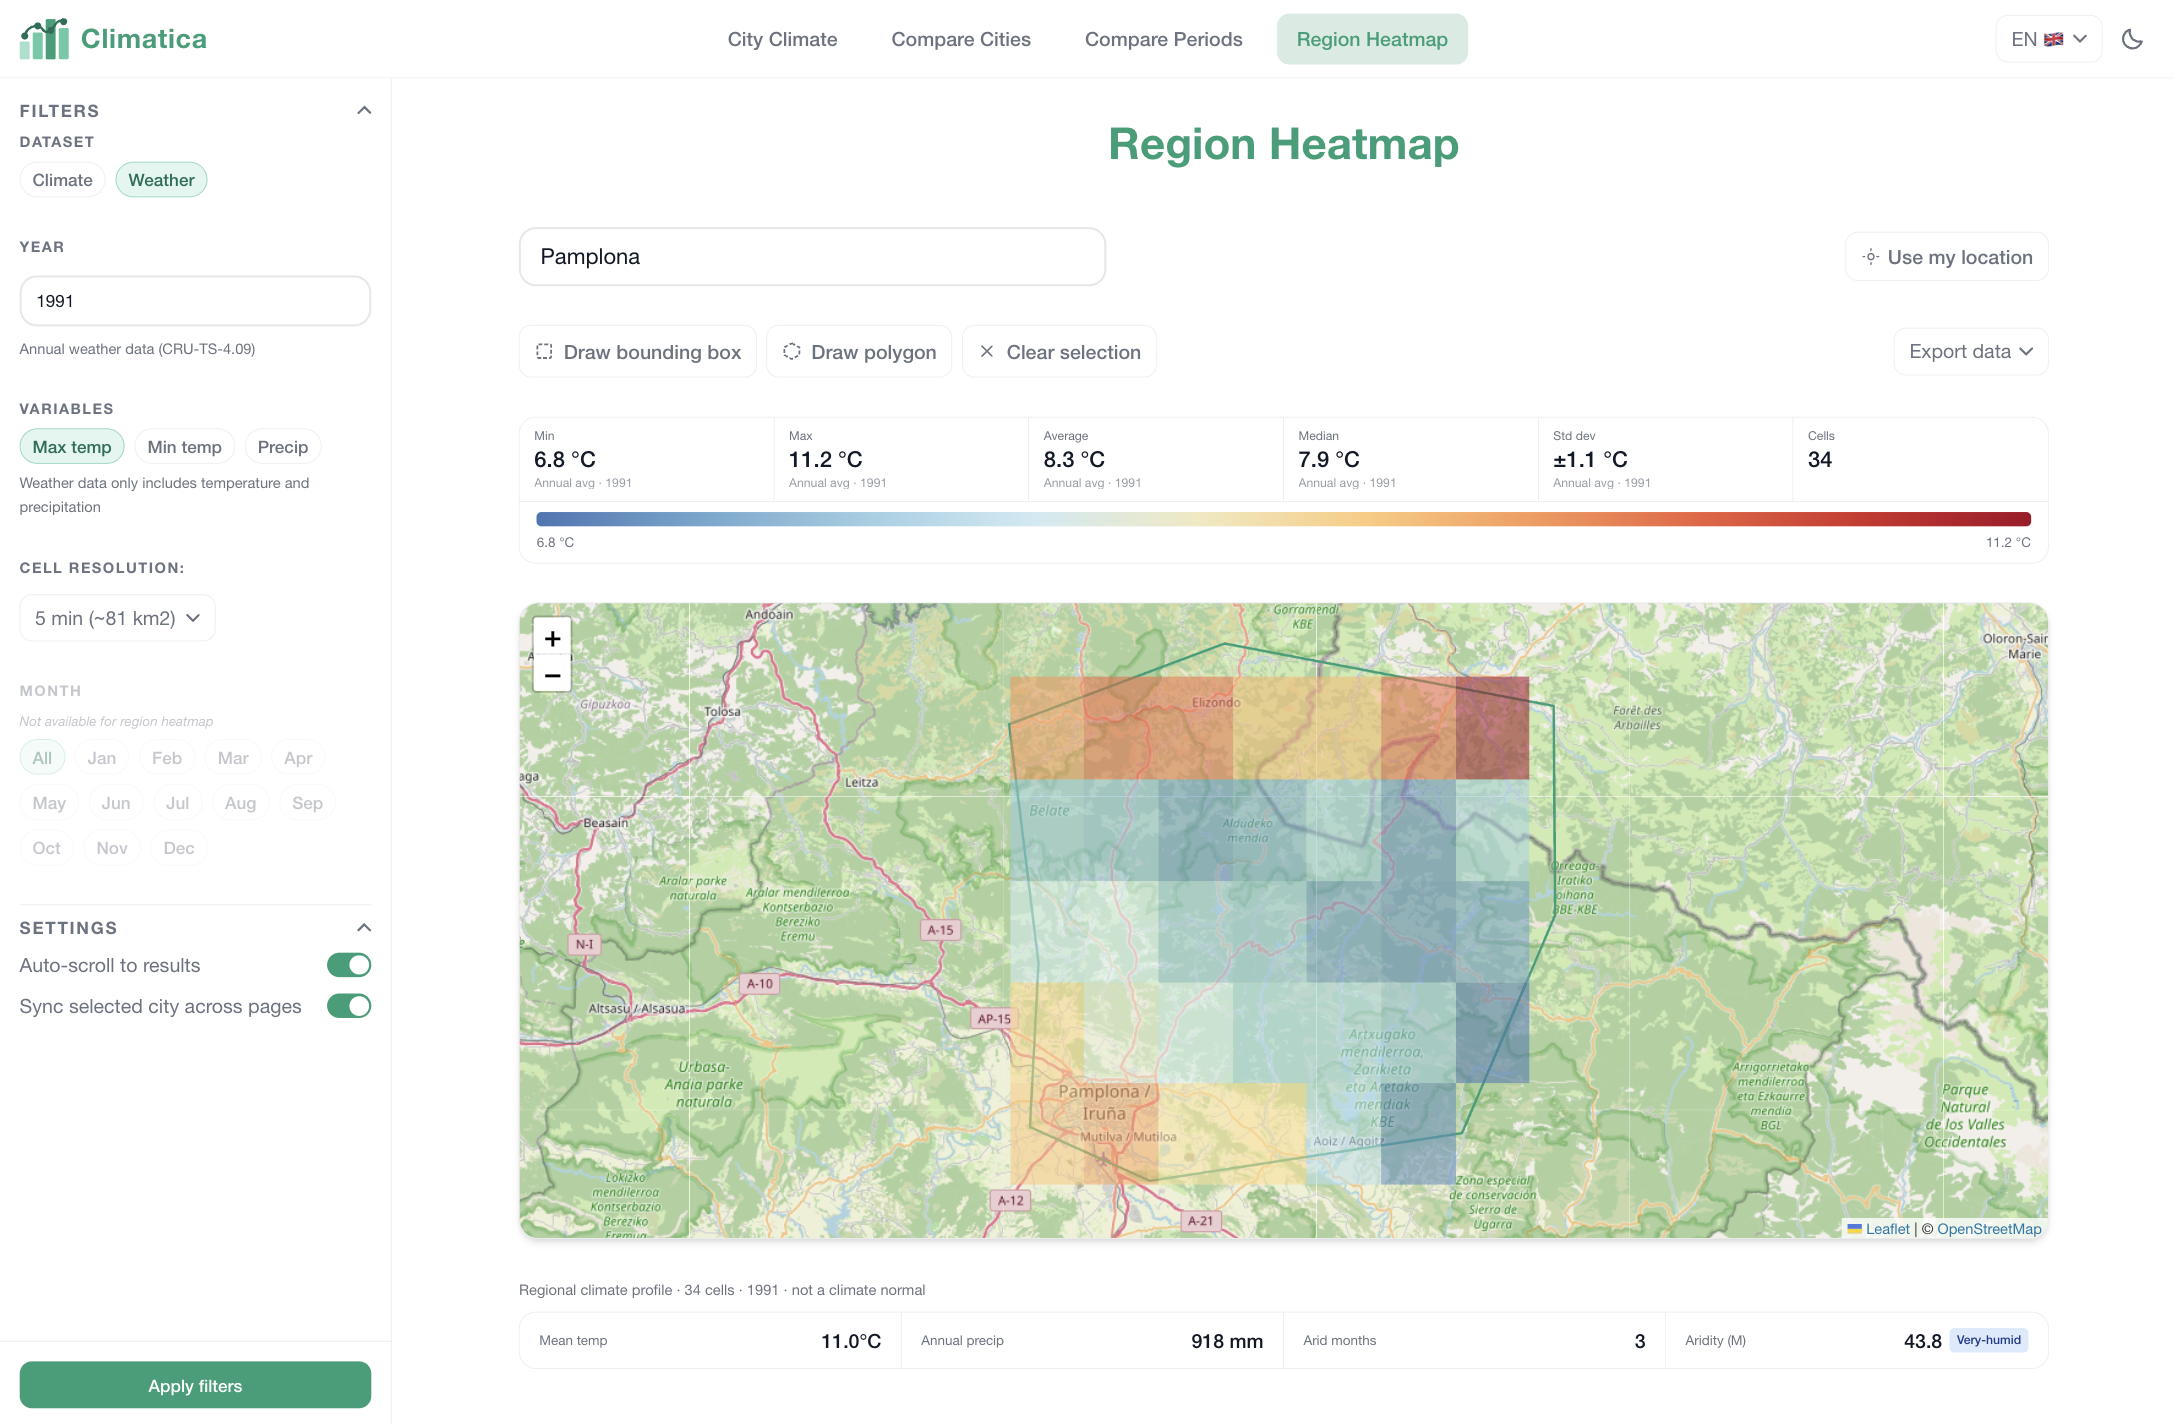
\includegraphics[width=\textwidth]{Images/climatica-demo-decline-heatmap.png}
  \caption{Region Heatmap page showing annual average maximum temperature
    across the Pyrenean foothills east of Pamplona (weather dataset, 1991).
    The thermal gradient from the warm Ebro valley lowlands (orange--red cells,
    $>$\,11\,$^\circ$C) to the cooler Pyrenean highlands (blue cells,
    $<$\,7\,$^\circ$C) is clearly resolved across 34 cells. The regional
    profile confirms a mean temperature of 11.0\,$^\circ$C and annual
    precipitation of 918\,mm (Martonne index 43.8, Very-humid).%
    \footnote{\url{https://climatica.gsic.uva.es/heat-map?dataset=weather&var=tmax%2Ctmin%2Cprec&grid=2.5m&year=1991&polygon=POLYGON%28%28-1.7405187919516065+42.8667978158502%2C+-1.7281560119783657+42.79830074711698%2C+-1.6347483410694652+42.758981410137366%2C+-1.4932631924868536+42.74788682662301%2C+-1.3971082371394707+42.90303023391967%2C+-1.3710090349737383+43.02867199453541%2C+-1.5921654322727588+43.06280215750196%2C+-1.788596269625318+43.02264705344673%2C+-1.7405187919516065+42.8667978158502%29%29}}}
  
  \label{fig:demo_decline_heatmap}
\end{figure}

\subsubsection{Outcome}

Within a single session, the ecologist has assembled a coherent body of
evidence linking the observed forest decline to a documented multi-decade
warming trend at the study site (+1.9\,$^\circ$C over 38 years), high
inter-annual variability in summer precipitation creating periodic drought
stress, and a spatially resolved thermal gradient that identifies the
lower-elevation, south-facing zones as the most vulnerable parts of the
landscape. This evidence base --- which would previously have required manual
extraction from WorldClim GeoTIFF files and custom scripting --- was assembled
interactively in approximately twenty minutes, using only a web browser and
no specialist software.

% * ─── 4.2 Methodology ─────────────────────────────────────────────────────────
\section{Evaluation Methodology}\label{EVAL_METHOD}

The evaluation was conducted as a user study on 3 June 2026 during a
presentation session at the Universidad de Valladolid in Palencia at the Yutera campus 
attended by students
from multiple European universities participating in an Erasmus+ programme.
All participants were domain users --- students enrolled in degree programmes
in forestry, environmental science, or biology --- rather than software
professionals, making them representative of Climatica's intended audience.

Each participant was given a brief live demonstration of the application and
then invited to explore it independently on their own device for approximately
ten minutes. At the end of the session they were asked to complete an online
questionnaire. The questionnaire comprised four parts:

\begin{enumerate}
  \item \textbf{Background questions} --- university, degree programme, year
    of study, and self-assessed knowledge level across six domains (climatology,
    GIS, data analysis, programming, databases, and general IT/web tools).
  \item \textbf{System Usability Scale (SUS)} --- the standard ten-item
    questionnaire~\cite{brooke1996sus} designed to produce a single usability
    score on a 0--100 scale.
  \item \textbf{Net Promoter Score (NPS)} --- a single question asking how
    likely the participant is to recommend Climatica to a friend or colleague,
    rated 0--10.
  \item \textbf{Open-ended questions} --- three free-text fields asking what
    the participant liked least, liked most, and would suggest as an
    improvement.
\end{enumerate}

Participation was voluntary and anonymous. Respondents were asked to confirm
their informed consent before proceeding. All 27 responses collected were
retained for analysis; no responses were excluded.

% * ─── 4.3 Participant Profile ─────────────────────────────────────────────────
\section{Participant Profile}\label{EVAL_PARTICIPANTS}

Twenty-seven students from ten European institutions completed the
questionnaire. The institutions represented included the Free University of
Bolzano (Italy), the University of Molise (Italy), the Warsaw University of
Life Sciences (Poland), the University for Sustainable Development Eberswalde
(Germany), and the Polytechnic Institute of Bragança (Portugal), among others.

The distribution across fields of study was strongly weighted towards
Forestry and Natural Resource Management (18 respondents, 67\%), followed by
Biology (6 respondents, 22\%), and Engineering, Earth Sciences, and Forest
Information Technology (one respondent each). The majority of respondents were
in their second or third year of study (13 and 6 respondents respectively).

Table~\ref{tab:knowledge} shows the self-reported knowledge levels across the
six assessed domains, expressed as means on a five-point scale
(0~=~None, 1~=~Basic, 2~=~Intermediate, 3~=~Advanced, 4~=~Expert). The
participant group was moderately experienced in climatology, GIS, and data
analysis --- the domains most directly relevant to Climatica's subject matter
--- but had limited programming and database backgrounds, consistent with a
target audience of domain specialists rather than software developers.

\begin{table}[H]
  \centering
  \caption{Self-reported knowledge levels of study participants
           (mean on a 0--4 scale; $n = 27$).}
  \label{tab:knowledge}
  \small
  \begin{tabular}{lcc}
    \toprule
    \textbf{Domain} & \textbf{Mean} & \textbf{Interpretation} \\
    \midrule
    Climatology and meteorology   & 2.00 & Intermediate \\
    GIS and geospatial data       & 2.22 & Intermediate--Advanced \\
    Data analysis \& visualisation & 2.00 & Intermediate \\
    Programming                    & 1.26 & Basic \\
    Databases                      & 1.37 & Basic--Intermediate \\
    General IT / web tools         & 1.56 & Basic--Intermediate \\
    \bottomrule
  \end{tabular}
  \normalsize
\end{table}

% * ─── 4.4 Usability Results ───────────────────────────────────────────────────
\section{Usability Results}\label{EVAL_SUS}

\subsection{System Usability Scale}\label{EVAL_SUS_SCORE}

The System Usability Scale (SUS)~\cite{brooke1996sus} is a ten-item Likert
questionnaire in which alternating items are positively and negatively worded.
The raw score for each respondent is computed as:

\[
  \text{SUS} = 2.5 \times \left[
    \sum_{i \in \text{odd}} (x_i - 1)
    + \sum_{i \in \text{even}} (5 - x_i)
  \right]
\]

where $x_i$ is the respondent's rating for item $i$ on a 1--5 scale. The
resulting score lies in the range $[0, 100]$.

The mean SUS score across all 27 respondents was \textbf{84.6} (median~90.0,
standard deviation~14.7, range~47.5--100.0). According to the adjective
rating scale proposed by Bangor et al.~\cite{bangor2009sus}, a score in the
range 80--90 is rated \emph{Excellent} and a score above 90 is rated
\emph{Best Imaginable}. Climatica's mean score of 84.6 therefore falls in the
\emph{Excellent} range and exceeds the widely cited industry average of
68~\cite{brooke1996sus}.

Table~\ref{tab:sus_dist} groups the individual scores by grade band using the
curved grading system of Sauro and Lewis~\cite{sauro2012sus}. Nineteen of the
27 respondents (70\%) awarded a score of 87.5 or higher, placing Climatica in
the A or A+ band for the majority of users. Three respondents (11\%) gave
scores below 65, suggesting that a minority of users encountered meaningful
usability barriers.

\begin{table}[H]
  \centering
  \caption{Distribution of individual SUS scores by grade band ($n = 27$).}
  \label{tab:sus_dist}
  \small
  \begin{tabular}{cclc}
    \toprule
    \textbf{Grade} & \textbf{Score range} & \textbf{Adjective} & \textbf{Count} \\
    \midrule
    A+ & $\geq 84.1$ & Best imaginable & 19 \\
    A  & 80.8--84.0  & Excellent       & 1  \\
    B  & 74.0--80.7  & Good            & 3  \\
    C  & 68.0--73.9  & OK              & 2  \\
    D  & 51.0--67.9  & Poor            & 0  \\
    F  & $< 51.0$    & Awful           & 2  \\
    \bottomrule
  \end{tabular}
  \normalsize
\end{table}

\subsection{Net Promoter Score}\label{EVAL_NPS}

The Net Promoter Score (NPS) question asked participants to rate, on a 0--10
scale, how likely they were to recommend Climatica to a friend or colleague.
Respondents scoring 9--10 are classified as \emph{promoters}, those scoring
7--8 as \emph{passives}, and those scoring 0--6 as \emph{detractors}. The NPS
is then computed as:

\[
  \text{NPS} = \frac{\text{promoters} - \text{detractors}}{n} \times 100
\]

Of the 27 respondents, 15 were promoters (9--10), 9 were passives (7--8), and
3 were detractors (0--6), yielding a mean recommendation score of 8.8 and an
NPS of \textbf{+44}. An NPS above 0 indicates that promoters outnumber
detractors; scores above 30 are generally considered good, and scores above 70
are considered excellent~\cite{reichheld2003nps}. Climatica's score of +44
therefore indicates a strong recommendation intent among the participant group.

% * ─── 4.5 Qualitative Feedback ────────────────────────────────────────────────
\section{Qualitative Feedback}\label{EVAL_QUAL}

\subsection{What Participants Liked Most}\label{EVAL_QUAL_LIKED}

The open-ended responses were analysed thematically. The most frequently
recurring theme across the 23 responses to the ``liked most'' question was
\textbf{ease of use and intuitiveness}. Representative comments included:
\emph{``I found it very straightforward to use and it provides very useful and
interesting data extremely fast''}; \emph{``I like how intuitive it is''}; and
\emph{``Very easy to use, you can get a lot of information out of it.''} This theme
appeared in approximately 80\% of responses, suggesting that the zero-friction
design goal described in Section~\ref{APP_REQ_NONFUNC} was successfully
perceived by users.

The second most prominent theme was \textbf{global data coverage and
accessibility}, mentioned by approximately 25\% of respondents. Several
highlighted the fact that climate data was available for any point on the
globe without requiring registration or local software:
\emph{``I found it very easy to use and I also like the fact that data is
in raster so you can have it at every point of the globe''}; 
\emph{``Access to data for any place in the world, fast results, visualisation 
of climographs and heatmaps.''}

A third theme was \textbf{the comparative and temporal views}, mentioned by
approximately 10\% of respondents. Several specifically mentioned the city
comparison and period comparison features as highlights:
\emph{``Comparison, having good visualisation of dataset''};
\emph{``The ability to analyse historical climate data and compare it with current
data allows us to understand and assess climate change.''}

\subsection{What Participants Liked Least}\label{EVAL_QUAL_DISLIKED}

Nineteen respondents answered the ``liked least'' question. The most commonly 
reported issue was \textbf{the PNG export alignment bug}:
several respondents from different devices (Windows PC, iPad) noted that text
and chart elements appeared shifted in exported PNG files relative to their
on-screen positions. This issue has since been resolved in a subsequent update
to the export pipeline.

The second reported concern was \textbf{the manual filter application step}.
Two respondents noted that they had to click ``Apply filters'' after changing
filter values, which felt unintuitive: \emph{``You have to click on Apply filters
again''}; \emph{``Auto-apply filters when clicking on them.''} This is a deliberate
design decision --- the draft filter pattern described in
Section~\ref{APP_ARCH_DRAFT} prevents expensive API calls from firing on every
individual filter change --- but the tradeoff was not immediately obvious to
all users.

Two respondents mentioned \textbf{heatmap loading performance} as a concern.
The heatmap page queries potentially thousands of pixel values from SCRAPI
and renders them as individual map overlays; at coarse resolutions this is fast,
but finer resolutions over large bounding boxes can take several seconds.

One technically sophisticated respondent raised the absence of \textbf{raw
data download}: \emph{``I like least that Climatica doesn't show raw data or let you
download it easily. Great visuals, but limited access to the underlying
numbers.''} Currently Climatica supports CSV and PNG export of chart data but
does not expose the raw SCRAPI response or the pixel value matrix.

\subsection{Suggested Improvements}\label{EVAL_QUAL_SUGGEST}

The most frequently requested improvement was \textbf{better export
functionality}: fixing the PNG alignment issue, adding SVG export reliability
across platforms, and providing raw data downloads. Several respondents also
requested \textbf{finer-grained time periods} --- specifically, 10-year climate
normals in addition to the existing 30-year normals, and non-overlapping
periods. One respondent suggested a \textbf{mobile application}, and another
asked for \textbf{additional language support} beyond the current three locales.

% * ─── 4.6 Discussion ──────────────────────────────────────────────────────────
\section{Discussion}\label{EVAL_DISCUSS}

\subsection{Interpretation of Results}\label{EVAL_DISCUSS_RESULTS}

The evaluation context adds weight to these results. As part of their course,
participants had previously prepared Walter-Lieth climatograms by hand for
several locations, using a set of CSV files circulated by Prof.\ Bravo. Two
days later, Climatica was presented to the same group, who were able to
reproduce --- and substantially extend --- the same analysis almost
automatically, within minutes rather than the hours required for manual
preparation. This direct before-and-after comparison likely contributed to
the strongly positive reception of the tool.

The quantitative results are encouraging. A mean SUS score of 84.6 places 
Climatica in the \emph{Excellent} range on
the Bangor et al.\ adjective rating scale (which translates numeric SUS
scores into verbal categories such as Excellent, Good, and Poor), well above
the industry average of 68. The NPS of +44 indicates that a
substantial majority of participants would recommend the tool to peers. Both
metrics suggest that Climatica successfully delivers on its primary design goal
of being accessible to non-specialist users without requiring GIS or programming
expertise.

The qualitative feedback reinforces this conclusion. The dominant theme in the
``liked most'' responses was ease of use, which was mentioned unprompted by
approximately 80\% of respondents. This is particularly meaningful given that
the participant group had intermediate knowledge of climatology and GIS but
limited programming and database backgrounds --- precisely the audience for
whom the application was designed. The contrast with the tools surveyed in
Chapter~\ref{REL} is evident: platforms such as NASA Giovanni and Copernicus
C3S offer greater scientific depth, but their learning curve excludes the kind
of users who found Climatica immediately accessible.

The three lowest SUS scores (47.5, 50.0, and 65.0) merit attention. Examining
the corresponding qualitative responses reveals different explanations. One
respondent with a low score reported finding parts of the navigation
``confusing'' and requested tutorials, suggesting a genuine discoverability
issue. A second reported slow loading and the heatmap stopping after the first
query, which points to a performance and state-management bug rather than a
design problem. The third low score came from a respondent who gave uniformly
low ratings without elaboration in the free-text fields, making the root cause
unclear.

\subsection{Limitations}\label{EVAL_DISCUSS_LIMITS}

Several limitations of this evaluation should be noted.

\textbf{Sample size and representativeness.} Twenty-seven respondents is a
reasonable number for a SUS study --- Tullis and Stetson~\cite{tullis2004sus}
showed that reliable SUS estimates can be obtained with as few as 12--14
participants --- but the sample was drawn from a single presentation event,
which limits its diversity. All participants were European university students
in natural science programmes; the results may not generalise to other user
groups such as secondary school students, urban planners, or researchers in
data-sparse regions.

\textbf{Evaluation duration.} Participants used the application for
approximately ten minutes before completing the questionnaire. Short exposure
times are standard in SUS studies but may not reveal usability issues that
only emerge with sustained use, such as the filter workflow friction reported
by some respondents.

\textbf{Device and browser variability.} The PNG export alignment issue was
reported by multiple respondents using different devices. The evaluation did
not systematically record device and browser information, so it is not possible
to determine whether the issue affected all platforms equally or was
concentrated in specific configurations.

\textbf{Data accuracy concerns.} Two respondents noted that the altitude
displayed for their city did not match their expectations, even at the highest
resolution. This is an inherent limitation of the WorldClim interpolation
methodology (described in Section~\ref{REL_WORLDCLIM_INTERP}): elevation values
are derived from a digital elevation model, and the 900\,m cell size of the
30-second grid means that local topographic variation within a cell is not
captured. This limitation is shared by all tools built on WorldClim data.

\subsection{Future Work}\label{EVAL_DISCUSS_FUTURE}

The evaluation results point to several concrete directions for future
development.

\textbf{Export improvements.} Fixing the PNG alignment issue and ensuring
consistent SVG export across platforms and browsers are the highest-priority
items based on frequency of mention. Adding a raw data download option --- a
CSV or JSON export of the full monthly pixel values --- would address the most
technically sophisticated user requests.

\textbf{Filter workflow.} Making filter changes take effect immediately,
without requiring an explicit ``Apply'' click, would satisfy the most commonly
raised workflow complaint. This would require redesigning the draft filter
pattern to debounce API calls rather than gate them behind a button.

\textbf{Additional climate periods.} One respondent suggested supporting
10-year normals and
non-overlapping period ranges would significantly expand the temporal analysis
capability. These features are technically feasible given the SCRAPI data model,
which exposes individual weather years from 1951 to 2024.

\textbf{Heatmap performance.} Two respondents reported slow loading on the
Region Heatmap page at fine resolutions. Before optimising the rendering
layer, it would be necessary to profile whether the bottleneck lies in the
SCRAPI API response time or in the client-side rendering of individual
\texttt{L.rectangle} overlays.

\textbf{Mobile support.} One respondent requested a mobile application;
another noted that PNG exports were misaligned on iPad. The current Next.js
deployment serves a responsive web interface, but the map drawing interactions
(bounding box and polygon) are not yet optimised for touch input.

\textbf{Extended language support.} Adding further locales beyond English,
Spanish, and Ukrainian would broaden accessibility. The \texttt{next-intl}
infrastructure already in place makes adding new locales straightforward;
the main effort is in translating the 233 keys per locale.